\textbf{{1.地址码}}

地址码用来指出该指令的源操作数的地址(一个或两个)、结果的地址及下一条指令的地址。这里的``地址''既可以是主存地址,也可以是寄存器地址,甚至还可以是I/O设备地址。但为了讲解方便,\textbf{一般都假设``地址''为``主存地址''。}

\textbf{(1)四地址指令}

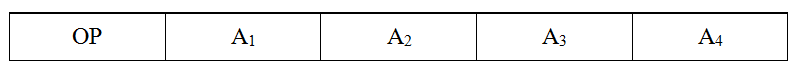
\includegraphics[width=3.12500in,height=0.26042in]{png-jpeg-pics/BF3E8018C03B31258CD9DADA3A9A3773.png}

在上图中,OP表示操作码;A1、A2分别为第一操作数和第二操作数地址;A3为存放运算结果的地址;A4为下一条指令的地址。

\textbf{(2)三地址指令}

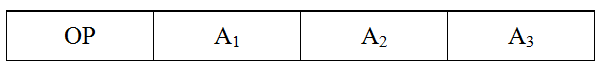
\includegraphics[width=2.70833in,height=0.30208in]{png-jpeg-pics/25068EE2D120888934E90DF46A69D0C6.png}

上图的指令可以完成操作(A1)OP(A2)→A3,后续指令的地址隐含在程序计数器中。

\textbf{(3)二地址指令}

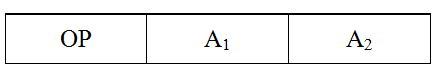
\includegraphics[width=2.29167in,height=0.37500in]{png-jpeg-pics/98ACA8040BA0254C8FACDC0EF0D6608A.png}

{{上图}{的指令可以完成操作}(A1)OP(A2)→A1或(A1)OP(A2)→A2。A1或A2既代表源操作数的地址,又代表存放本次运算结果的地址。}

\textbf{(4)一地址指令}

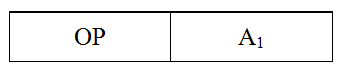
\includegraphics[width=1.96875in,height=0.39583in]{png-jpeg-pics/20F9250079D6870C31C1E6D5AD378D82.png}

如果其中一个操作数能隐藏在运算器的ACC就好了,这样取其中一个源操作数就可以直接在ACC中进行了,而且仅仅需要访问一次存储器取另外一个源操作数就够了。

\textbf{(5)零地址指令}

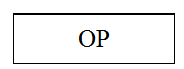
\includegraphics[width=1.14583in,height=0.42708in]{png-jpeg-pics/B1D45AE4B9EE447256AF80A41EBC9101.png}

确实有些指令还是可以进行优化的,如停机指令、空操作指令等是不需要地址码的,因此零地址指令产生了。如上图。

{\textbf{2.操作码}}

上一个知识点中提到过,\textbf{操作码被分为定长操作码和不定长操作码。}

定长操作码指令是在指令字的最高位部分分配固定的若干位表示操作码。对于具有n位操作码字段的指令系统,最多能够表示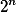
\includegraphics[width=0.16667in,height=0.12500in]{texmath/e538e52n}条指令。
